\newpage
\section{Introduction}
\label{sec:introduction}

% state the learning objective 

The objective of this laboratory assignment is to analyze a RC circuit to find the natural and forced response as well as doing a frequency analysis. Furthermore, it is asked to run a simulation using NgSpice to detect small diferences between the different approaches and understand why said differences happen. The circuit can be seen in Figure~\ref{fig:circuit}.

In Section~\ref{sec:analysis}, a theoretical analysis of the circuit is
presented. In Section~\ref{sec:simulation}, the circuit is analysed by
simulation and the results are compared to the theoretical results obtained in
Section~\ref{sec:analysis}. The conclusions of this study are outlined in
Section~\ref{sec:conclusion}.


\bigskip 

\begin{figure}[!ht] \centering
\caption{RC Circuit with alternate voltage source ($V_s$), linear dependent sources ($V_d$-linear current controlled voltage source and $I_b$-linear voltage controlled current source) and capacitor $C$}
\squeezeup 
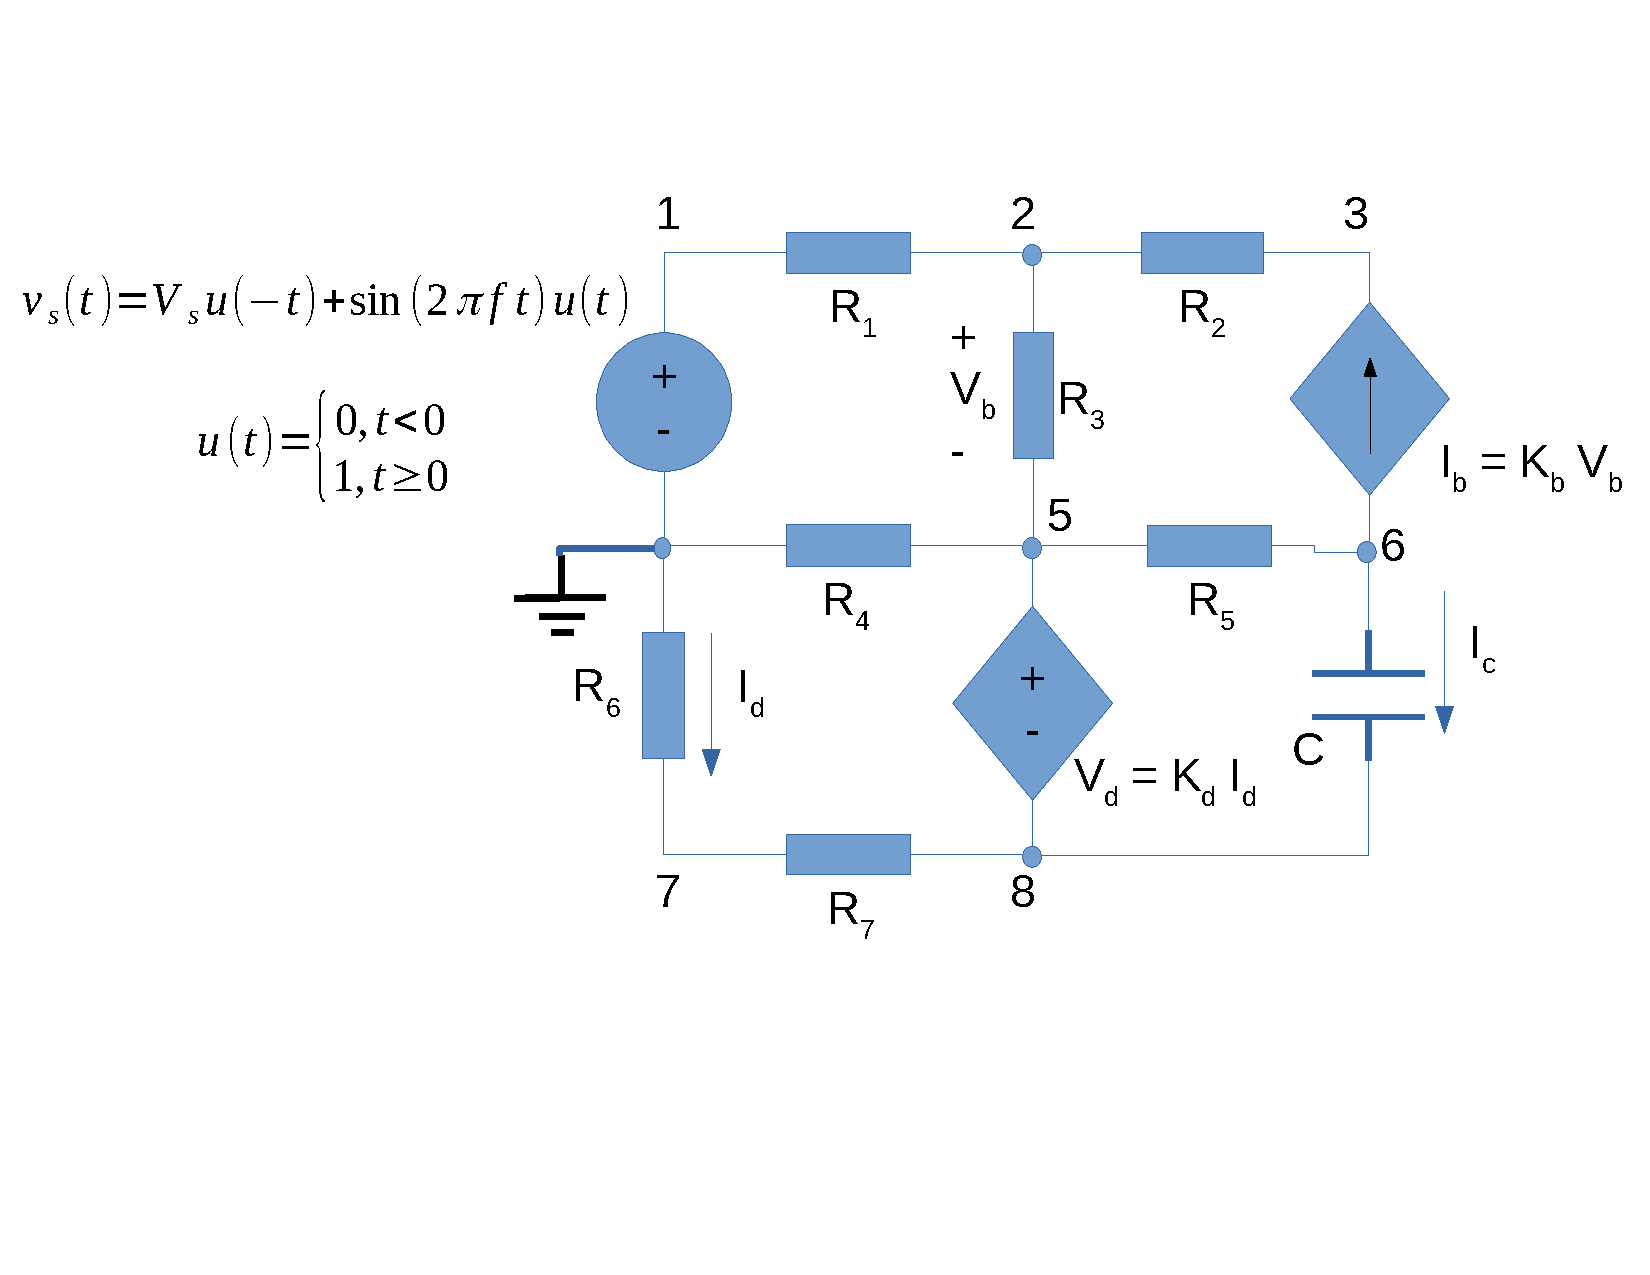
\includegraphics[width=0.9\textwidth, scale=1.0]{circuit.pdf}
\squeezeup 
\squeezeup 
\squeezeup 
\squeezeup 
\label{fig:circuit}
\end{figure}
The values given for this report can be found in table~\ref{tab:op1}(Obtained with the number $\partialinput{21}{21}{data.txt}$). 

\begin{table}[hb]
  \centering
  \begin{tabular}{|l|r|}
    \hline    
    {\bf Name} & {\bf Values} \\ \hline
    @c1[i] & 0.000000e+00\\ \hline
@gib[i] & -2.45467e-04\\ \hline
@r1[i] & -2.34492e-04\\ \hline
@r2[i] & -2.45467e-04\\ \hline
@r3[i] & -1.09744e-05\\ \hline
@r4[i] & -1.22007e-03\\ \hline
@r5[i] & 2.454667e-04\\ \hline
@r6[i] & 9.855785e-04\\ \hline
@r7[i] & 9.855785e-04\\ \hline
v1 & 5.242048e+00\\ \hline
v2 & 5.002985e+00\\ \hline
v3 & 4.499645e+00\\ \hline
v5 & 5.036927e+00\\ \hline
v6 & 5.789615e+00\\ \hline
v7 & -1.98352e+00\\ \hline
v8 & -2.97405e+00\\ \hline
v9 & 0.000000e+00\\ \hline
v(v5,v2) & 3.394244e-02\\ \hline
v(v8,v5) & -8.01098e+00\\ \hline

  \end{tabular}
  \caption{Values obtained by using the Python program that can be found in folder $python$.}
  \label{tab:op1}
\end{table}


